\section{Results}

\subsection{Qualitative investigation of the relationship between inoculum concentration and macro-morphology}

An initial \lq range-finding' investigation into the effect of inoculum concentration on the macroscopic form of \emph{A. oryzae} was performed to study the effect of spore concentration on pellet formation. The initial selection of spore concentrations was based on a review of studies involving shake-flask culturing of \emph{Aspergilli} \cite{papagianni2002,xu2000,papagianni2006a,carlsen1996a}. Inoculum concentrations of less than \inoc{1}{7} frequently resulted in the formation of large agglomerates of biomass (Fig.~\ref{fig:QualInoc}). Based on Pirt's theory of pellet growth, which states that actively-growing hyphae are restricted to a narrow region (estimated as \mic{$<\sim 350$} deep in \emph{A. oryzae} \cite{carlsen1996a}) at a pellet's surface \cite{pirt1966}, such large agglomerates would be expected to contain a very high proportion of diffusion-limited biomass. Furthermore, such agglomerates do not lend themselves to meaningful morphological analysis. While pellets were sometimes produced with an inoculum of \inoc{1}{6}, the inherent variability of the submerged culture format resulted in frequent biomass aggregation at this inoculum level (Fig.~\ref{fig:10x6a}). A minimum inoculum concentration of \inoc{1}{7} was therefore chosen for subsequent study of \emph{A. oryzae} in submerged culture to maximise morphological reproducibility between flasks.

\begin{figure}[tb]
	\centering
	\subfloat[]{\label{fig:10x4}\fbox{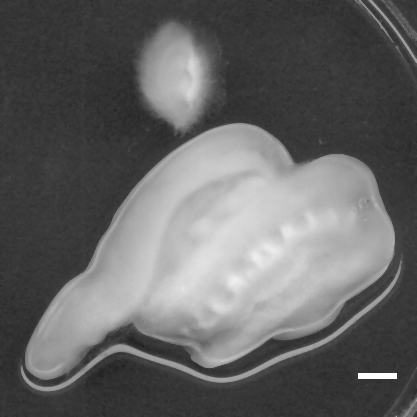
\includegraphics[width=4cm]{../C5/10x4}}}
	\hspace{0.5cm}
	\subfloat[]{\label{fig:10x6a}\fbox{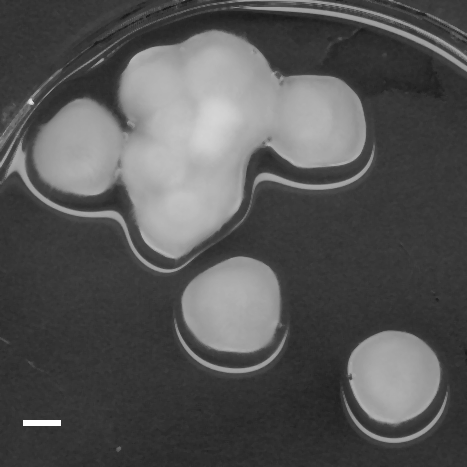
\includegraphics[width=4cm]{../C5/10x6a}}}
	\hspace{0.5cm}
	\subfloat[]{\label{fig:10x7}\fbox{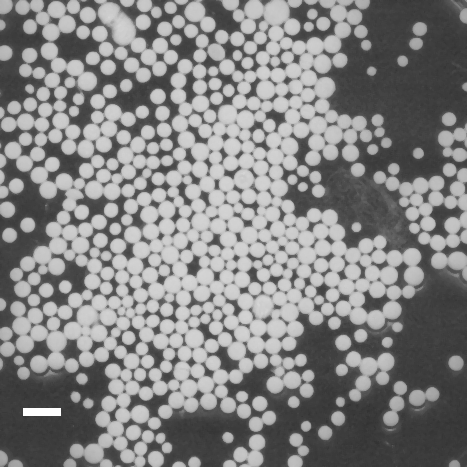
\includegraphics[width=4cm]{../C5/10x7}}}
	\caption{Variation in macroscopic morphological forms of \emph{A. oryzae} for inoculum concentrations of (a) $1 \times 10^4$, (b) $1 \times 10^6$ and (c) \inoc{1}{7} ($34.1 \pm 5.8$\% viability). Bars: 5 mm. }
	\label{fig:QualInoc}
\end{figure}

\subsection{Characterisation of morphological development and product formation in submerged culture over time}

\begin{figure}[htbp]
	\centering
	\captionsetup[subfloat]{position=top}
	\subfloat[]{\label{fig:BasicFermDp} \pstool[width=9.6cm]{../C5/BasicFermDp}{
		\psfrag{T}[Bc]{\al \hspace{2mm} Time (h)}
		\psfrag{D}[Bc]{\al \hspace{1mm} $\Dp$ (mm)}
		\psfrag{B}[Bc]{\al \hspace{1mm} DCW (\omgml)}}
	}
	\\
	\captionsetup[subfloat]{position=bottom}
	\subfloat[]{\label{fig:PelletMorpha}\fbox{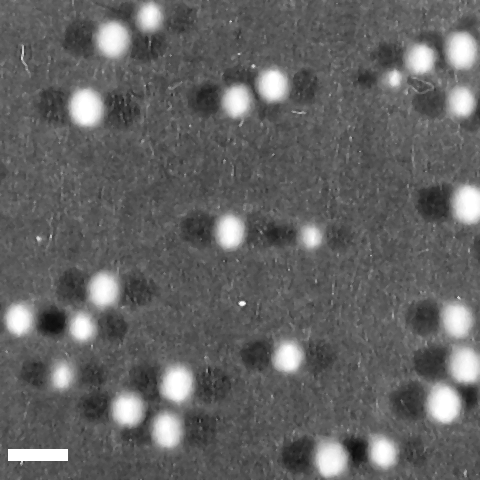
\includegraphics[width=3cm]{../C5/PelletMorpha}}}
	\hspace{0.5cm}
	\subfloat[]{\label{fig:PelletMorphb}\fbox{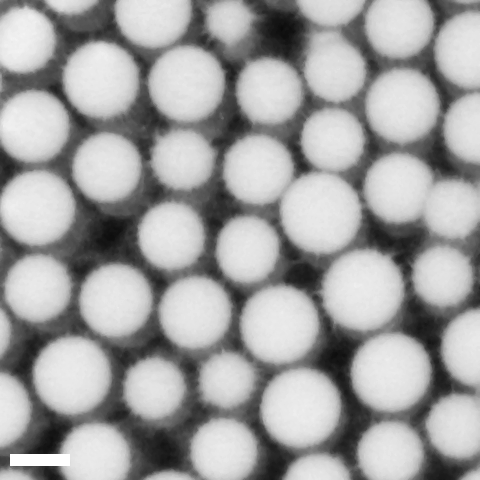
\includegraphics[width=3cm]{../C5/PelletMorphb}}}
	\hspace{0.5cm}
	\subfloat[]{\label{fig:PelletMorphc}\fbox{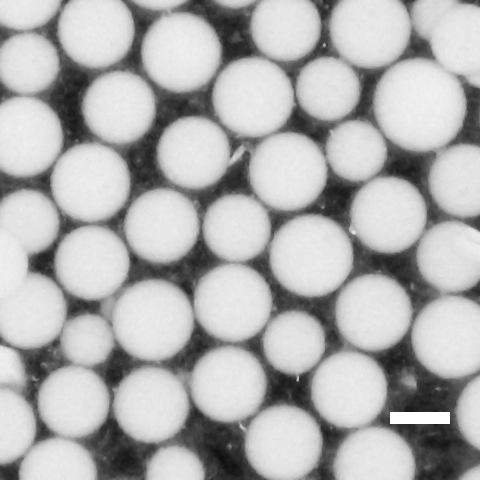
\includegraphics[width=3cm]{../C5/PelletMorphc}}}
	\\
	\subfloat[]{\label{fig:PelletMorphd}\fbox{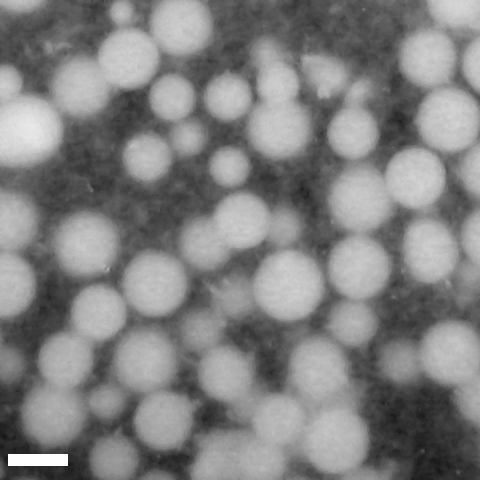
\includegraphics[width=3cm]{../C5/PelletMorphd}}}
	\hspace{0.5cm}
	\subfloat[]{\label{fig:PelletMorphe}\fbox{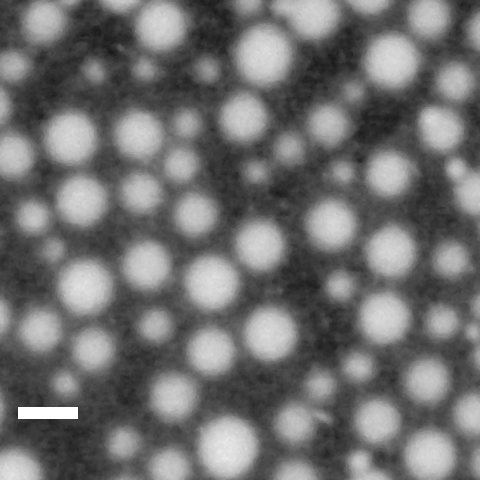
\includegraphics[width=3cm]{../C5/PelletMorphe}}}
	\caption{(a) Variation in mean pellet diameter ($\Dp$; $\bullet$) and dry-cell weight (DCW; $\bs$) during a \lq standard' submerged fermentation of \emph{A. oryzae}. Error bars represent 95\% confidence intervals. Images of macro-morphology were captured at (b) 24, (c) 45, (d) 72, (e) 96 and (f) 168~hours (Bars: 2 mm). Organism cultivated in BM (pH~7.0) supplemented with yeast extract (0.5 \% w/v) and starch (0.8 \% w/v). Each data point represents a single flask terminated at the indicated time. All flasks incubated at \celc{25}, $\mbox{spore viability}=34.1 \pm 5.8$\%.}
	\label{fig:BasicFermPellets}
\end{figure}

The variation in the macro-morphology of \emph{A. oryzae} was evaluated over the course of a 7-day shake-flask fermentation (Fig.~\ref{fig:BasicFermDp}), the development of which is illustrated in Figure~\ref{fig:PelletMorpha} to \ref{fig:PelletMorphe}. The pellets attained their maximum diameter 45 -- 72~hours post-inoculation and appeared to degrade from this point on. This may have been a result of nutrient exhaustion (depletion of starch was confirmed by observing the reaction between samples of fermentation broth and Lugol's iodine - not shown) and a subsequent weakening of cell structure, resulting in hyphal fragmentation at the pellet periphery; low levels of substrate have previously been demonstrated to lead to increased vacuolation and subsequent hyphal fragmentation in \emph{A.~niger} \cite{papagianni1999}. This fragmentation resulted in a large increase in mycelial \lq clumps' in the media, depicted by the \lq cloudy' nature of Figure~\ref{fig:PelletMorphd} and \ref{fig:PelletMorphe}. These clumps were observed using light microscopy, but analysis and quantification was not possible as staining with lactophenol cotton blue proved problematic (Fig.~\ref{fig:LPCBWetStain}).

\begin{figure}[bt]
	\centering
	\subfloat[]{\label{fig:PartlyStainedHypha}\fbox{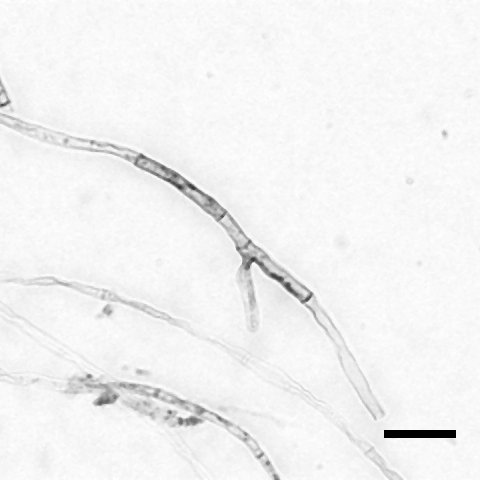
\includegraphics[width=5cm]{../C5/PartlyStainedHypha}}}
	\hspace{0.5cm}
	\subfloat[]{\label{fig:UnstainedHypha}\fbox{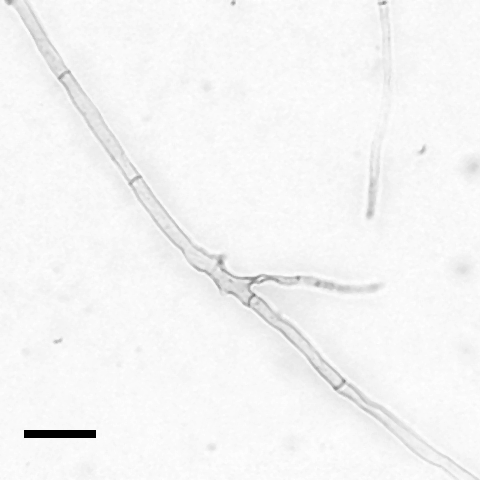
\includegraphics[width=5cm]{../C5/UnstainedHypha}}}
  \caption{Conventional lactophenol cotton blue \lq wet-mounts' of 72-hour-old samples showed limited stain uptake (a), or in some cases, none at all (b). Bars: \mic{25}.}
  \label{fig:LPCBWetStain}
\end{figure}

The assessment of pellet sizes is complicated somewhat in this scenario as accurate image segmentation (separation of pellets from background) is more difficult and an evaluation of pellet size alone does not provide complete morphological quantification of the organism. Up to 72~hours post-inoculation, biomass exists in almost exclusively pelleted form and, as such, a measure of the size of these pellets provides an accurate representation of the organism's phenotype. However, beyond this point, a variety of structures are present, the smallest of which may be excluded from the analysis by virtue of the limited resolution of the scanner (and limited stain uptake), and therefore the mean size of biomass elements (expressed as mean pellet diameter) is possibly over-estimated beyond 72~hours.

The fragmentation of pellets is further illustrated in Figure~\ref{fig:DpDist}. Overall pellet diameter of a sample population increased from 24 -- 45~hours and remained relatively constant until 72~hours. Thereafter, a large increase in the number of objects with an equivalent diameter below $\sim 2$~mm coincided with a reduction in the number of objects with diameters above $\sim 3$~mm. This suggests that larger pellets had begun to fragment, forming smaller pellet-like structures and clumps.

\begin{figure}[htbp]
	\centering
	\subfloat{\label{fig:DpDist24h}\pstool[width=6.5cm]{../C5/DpDistDay2}{
		\psfrag{F}[Bc]{\al \% Frequency}
		\psfrag{D}[tc]{\al \hspace{1mm} $\Dp$ (mm)}
		\psfrag{H}[Bc]{\bf 24 h}}}
	\hspace{1cm}
	\subfloat{\label{fig:DpDist45h}\pstool[width=6.5cm]{../C5/DpDistDay3}{
		\psfrag{F}[Bc]{\al \% Frequency}
		\psfrag{D}[tc]{\al \hspace{1mm} $\Dp$ (mm)}
		\psfrag{H}[Bc]{\bf 45 h}}}
	\\
	\subfloat{\label{fig:DpDist72h}\pstool[width=6.5cm]{../C5/DpDistDay4}{
		\psfrag{F}[Bc]{\al \% Frequency}
		\psfrag{D}[tc]{\al \hspace{1mm} $\Dp$ (mm)}
		\psfrag{H}[Bc]{\bf 72 h}}}
	\hspace{1cm}
	\subfloat{\label{fig:DpDist96h}\pstool[width=6.5cm]{../C5/DpDistDay5}{
		\psfrag{F}[Bc]{\al \% Frequency}
		\psfrag{D}[tc]{\al \hspace{1mm} $\Dp$ (mm)}	
		\psfrag{H}[Bc]{\bf 96 h}}}
	\\
	\subfloat{\label{fig:DpDist168h}\pstool[width=6.5cm]{../C5/DpDistDay8}{
		\psfrag{F}[Bc]{\al \% Frequency}
		\psfrag{D}[tc]{\al \hspace{1mm} $\Dp$ (mm)}	
		\psfrag{H}[Bc]{\bf 168 h}}}
  \caption{Variation in distributions of pellet diameter ($\Dp$) over time in shake-flask cultures of \emph{A.~oryzae} ($44 \leq n \leq 357$). Cultivation conditions were as described in Figure~\ref{fig:BasicFermPellets}.}
  \label{fig:DpDist}
\end{figure}

In their study of \emph{A. oryzae} in the form of pellets, Carlsen and colleagues estimated that oxygen limitation set in 23~hours post-inoculation, when the pellets were approximately 600 -- \mic{800} in diameter \cite{carlsen1996a}. The pellets continued to increase in size until approximately 35~hours, when mean pellet diameter began to decline, the number of pellets per unit volume increased rapidly and an increase in ethanol concentration was noted. No ethanol was detected in cultures grown as freely dispersed hyphal elements, indicating ethanol production was limited to the dense pellet core, where anaerobic conditions predominated. This may suggest that autolysis contributed to the decline in pellet diameter and biomass concentration illustrated in Figure~\ref{fig:BasicFermPellets}, given that the measured diameters were well in excess of those reported by Carlsen and colleagues.

The rate of $\alpha$-amylase production slowed considerably once maximum pellet diameter and maximum biomass levels had been attained (Fig.~\ref{fig:BasicFermBiochem}), suggesting that production of this enzyme is primarily growth-associated. Carlsen and colleagues demonstrated a similar concurrent increase in biomass and $\alpha$-amylase production in batch cultivations of \emph{A. oryzae} (specific $\alpha$-amylase production was constant) \cite{carlsen1996a} and it was later reported that $\alpha$-amylase synthesis was closely coupled to the growth of the fungus \cite{carlsen1996b}. However, Spohr and colleagues found that the specific $\alpha$-amylase secretion rate seemed to decrease with time during batch cultivation, although no explanation was offered for this observation \cite{spohr1997}. Exhaustion of starch (an inducer of $\alpha$-amylase production in \emph{A. oryzae} \cite{agger2002}) may have been responsible for the decline in $\alpha$-amylase production observed here. It is also possible that the presence of glucose, resulting from total starch degradation, had repressed $\alpha$-amylase production, as has been previously documented \cite{carlsen1996b}. Peak specific $\alpha$-amylase activity (IU mg\sp{-1} extra-cellular protein) occurred at 45~hours (Fig.~\ref{fig:BasicFermSpec}), coinciding with peaks in pellet diameter and biomass levels and indicating a reduction in $\alpha$-amylase production beyond this point in the fermentation.

\begin{figure}[htbp]
	\centering
	\captionsetup[subfloat]{position=top}
	\subfloat[]{\label{fig:BasicFermBiochem} \pstool[width=10.5cm]{../C5/BasicFermBiochem}{
		\psfrag{d}[cc]{\al \hspace{1mm} $\alpha$-amylase activity (IU ml\sp{-1})}
		\psfrag{T}[Bc]{\al \hspace{2mm} Time (h)}
		\psfrag{P}[cc]{\al \hspace{1mm} Extra-cellular protein conc. (\omgml)}}
	}
	\\
	\subfloat[]{\label{fig:BasicFermSpec} \pstool[width=10.5cm]{../C5/BasicFermSpec}{
		\psfrag{A}[Bc]{\al \hspace{1mm} Specific $\alpha$-amylase activity (IU mg\sp{-1})}
		\psfrag{T}[Bc]{\al \hspace{2mm} Time (h)}}
	}
	\caption{Typical submerged fermentation of \emph{A. oryzae} showing (a) $\alpha$-amylase activity ($\bt$), extra-cellular protein concentration ($\bl$) and (b) specific $\alpha$-amylase activity (IU mg\sp{-1} protein). Cultivation conditions were as described in Figure~\ref{fig:BasicFermPellets}.}
	\label{fig:BasicFerm}
\end{figure}

The results of these preliminary experiments provided a baseline understanding of the development of \emph{A. oryzae} in shake-flask culture and permitted the design of further experiments examining the relationship between morphology and $\alpha$-amylase production. This result suggested that a sampling time of 45 -- 72~hours was optimal for comparing different shake-flask conditions, given that growth and primary metabolite production of the organism had peaked by this time.

\subsection{Investigation into the use of solid supports in submerged fermentation}

In an attempt to garner an insight into the early stages of hyphal development in liquid media, initial work on the characterisation of submerged fermentations was combined with the assay described in Chapter~\ref{ch:NitroAssay} to provide a novel \lq mixed-phase' cell-immobilisation culture format. In addition to possible facilitation of micro-morphological observation, the use of solid supports in submerged culture has shown potential for both increased metabolite yield \cite{papagianni2004} and differential protein expression \cite{bigelis2006}. A series of shake-flask fermentations were conducted to determine the effect of starch concentration on both the mixed-phase and conventional submerged systems.

When cultivated in the mixed phase format, virtually all biomass remained adhered to the membrane (Fig.~\ref{fig:MixedMorpha} to \ref{fig:MixedMorphd}) - the absence of mycelial elements or pellets in the broth was confirmed by both visual and microscopic inspection. However, acquiring any morphological data from such agglomerates, other than projected area (a proxy indicator of biomass levels), was not possible. Other authors have availed of scanning electron microscopy to visualise immobilised biomass, but the resultant morphological descriptions were qualitative in nature \cite{papagianni2004}. However, it is interesting to note the lack of a filamentous or annular region around the periphery of the agglomerates, as would often be visible on pellets, which may suggest that peripheral hyphae were compacted by fluid eddies, as described by Rodr\'{i}guez Porcel and colleagues \cite{rodriguezporcel2005}.

\begin{figure}[tb]
	\centering
	\subfloat[0.0\%]{\label{fig:MixedMorpha}\fbox{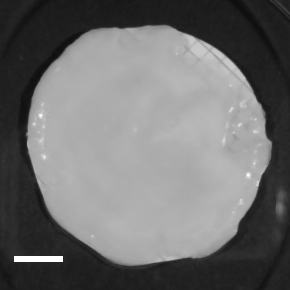
\includegraphics[width=3.1cm]{../C5/MixedMorpha}}}
	\hspace{0.25cm}
	\subfloat[0.8\%]{\label{fig:MixedMorphb}\fbox{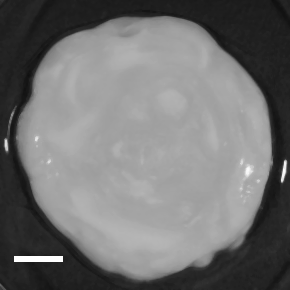
\includegraphics[width=3.1cm]{../C5/MixedMorphb}}}
	\hspace{0.25cm}
	\subfloat[1.6\%]{\label{fig:MixedMorphc}\fbox{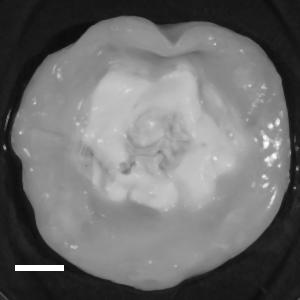
\includegraphics[width=3.1cm]{../C5/MixedMorphc}}}
	\hspace{0.25cm}
	\subfloat[3.2\%]{\label{fig:MixedMorphd}\fbox{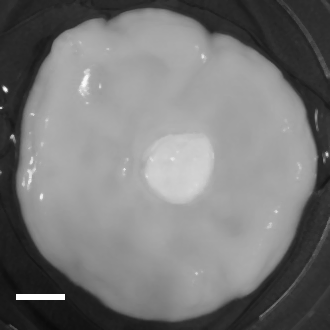
\includegraphics[width=3.1cm]{../C5/MixedMorphd}}}
	\\
\subfloat[0.0\%]{\label{fig:VaryCPelletMorpha}\fbox{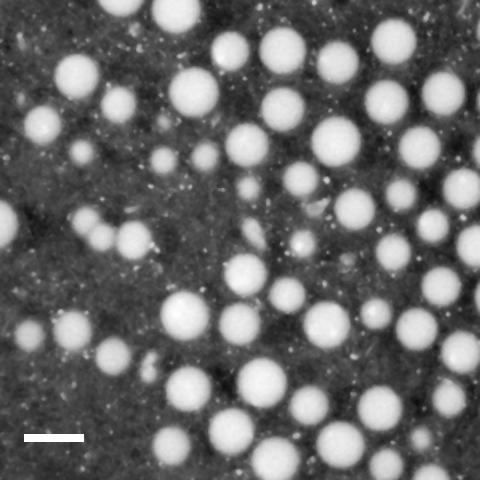
\includegraphics[width=3.1cm]{../C5/VaryCPelletMorpha}}}
\hspace{0.25cm}
\subfloat[0.8\%]{\label{fig:VaryCPelletMorphb}\fbox{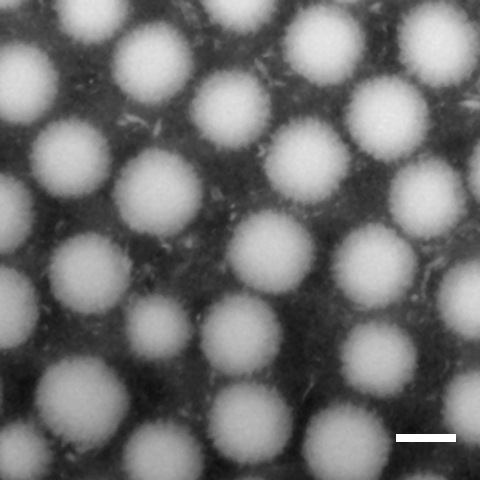
\includegraphics[width=3.1cm]{../C5/VaryCPelletMorphb}}}
\hspace{0.25cm}
\subfloat[1.6\%]{\label{fig:VaryCPelletMorphc}\fbox{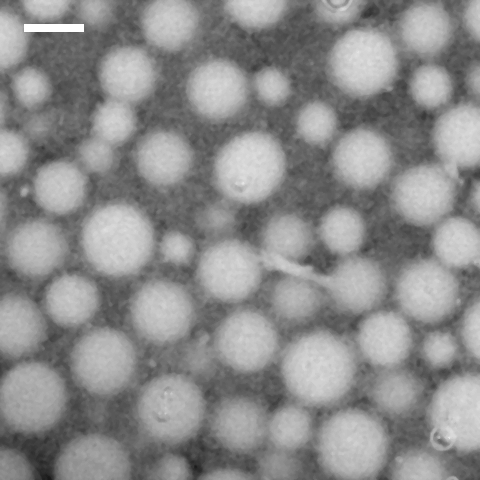
\includegraphics[width=3.1cm]{../C5/VaryCPelletMorphc}}}
\hspace{0.25cm}
\subfloat[3.2\%]{\label{fig:VaryCPelletMorphd}\fbox{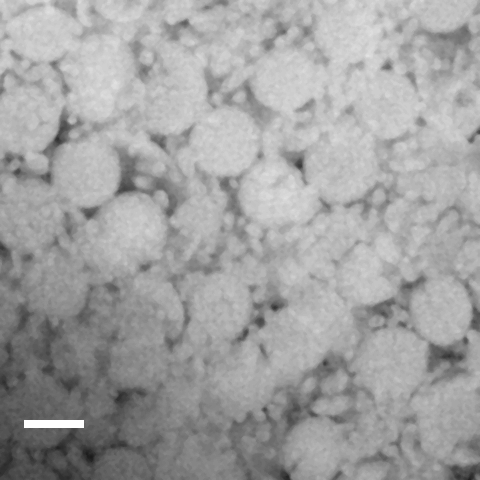
\includegraphics[width=3.1cm]{../C5/VaryCPelletMorphd}}}
  \caption{Morphological form of \emph{A. oryzae} 120~hours post-inoculation in mixed-phase (\lq a' - \lq d', bars: 10~mm) and submerged fermentations (\lq e' - \lq h', bars: 3~mm) supplemented with the indicated starch concentrations (w/v). Following incubation of membrane culture on SDA for the mixed-phase system, the organism was cultivated in BM (pH~7.0) supplemented with yeast extract (0.5\% w/v) and starch (at the indicated concentrations). All flasks and membranes were inoculated with \inoc{1}{7} ($34.1 \pm 5.8$\% viability).}
  \label{fig:VaryCMorph}
\end{figure}

Increasing substrate concentration was found to have a significant impact on the gross, macroscopic form of the organism in the submerged format (Fig.~\ref{fig:VaryCPelletMorpha} to \ref{fig:VaryCPelletMorphd}), with dispersed growth becoming more common as the substrate concentration was increased, complicating the quantification of the resulting macro-morphologies. It is possible that this dispersed growth may be explained by the presence of a greater number of \lq growth centres', provided for by the increased substrate concentration. Starch is not completely soluble at room temperature and, as its concentration in the media was increased, it is possible that a greater number of starch \lq particles' were present in the media. These may have provided sites onto which germinating spores adhered themselves, resulting in a more dispersed growth at higher starch concentrations. Such a mechanism has previously been documented in the culturing of \emph{A.~oryzae} \cite{truong2004} and \emph{A.~awamori} \cite{cui1998a} in complex media containing solid particles. Alternatively, the increase in viscosity that resulted from increasing substrate concentration may have been responsible for this observed change in biomass distribution. Indeed it has been reported that regulating apparent broth viscosity (through the addition of xanthan gum) resulted in a decrease in the volume of \emph{Streptomyces hygroscopicus} var. \emph{geldanus} pellets \cite{ocleirigh2005}. In this study, a microscopic examination was complicated by the presence of starch particles, particularly at higher concentrations, which obscured the field of view and made the isolation of individual hyphae for analysis difficult to achieve.

\begin{figure}[htbp]
	\centering
	\captionsetup[subfloat]{position=top}
	\subfloat[]{\label{fig:AaDCWS}\pstool[width=10.3cm]{../C5/AaDCWS}{
		\psfrag{S}[Bc]{\al \hspace{2mm} \% Starch (w/v)}
		\psfrag{D}[bc]{\al \hspace{1mm} DCW (\omgml);}
		\psfrag{d}[cc]{\al \hspace{1mm} $\alpha$-amylase activity (\IUml)}
		\psfrag{P}[Bc]{\al \hspace{1mm} Extra-cellular protein conc. (\omgml)}}	
	}
	\\
	\subfloat[]{\label{fig:VaryCMixed}\pstool[width=10.3cm]{../C5/VaryCMixed}{
		\psfrag{S}[Bc]{\al \hspace{2mm} \% Starch (w/v)}
		\psfrag{D}[bc]{\al \hspace{1mm} DCW (\omgml);}
		\psfrag{d}[cc]{\al \hspace{1mm} $\alpha$-amylase activity (\IUml)}
		\psfrag{P}[Bc]{\al \hspace{1mm} Extra-cellular protein conc. (\omgml)}}
	}
  \caption{Dry-cell weight (DCW; $\bs$), $\alpha$-amylase activity ($\bt$) and extra-cellular protein concentration ($\bl$) for varying starch concentrations in the (a) submerged and (b) mixed-phase fermentation of \emph{A. oryzae} 120~hours post-inoculation. Cultivation conditions were as described in Figure~\ref{fig:VaryCMorph}. Error bars represent standard deviation of two independent results.}
  \label{fig:VaryC}
\end{figure}

\begin{figure}[tb]
	\centering
	\pstool[width=10.5cm]{../C5/VaryCAAperDCW}{
		\psfrag{S}[Bc]{\al \hspace{2mm} \% Starch (w/v)}
		\psfrag{A}[Bc]{\al \hspace{1mm} $\alpha$-amylase activity per DCW (IU mg\sp{-1})}}
  \caption{$\alpha$-amylase activity per unit dry-cell weight for varying starch concentrations in the submerged ($\bs$) and mixed-phase fermentation ($\square$) of \emph{A. oryzae} 120~hours post-inoculation. Cultivation conditions were as described in Figure~\ref{fig:VaryCMorph}. Error bars represent standard deviation of two independent results.}
  \label{fig:VaryCAAperDCW}
\end{figure}

A direct relationship was found between substrate concentration and biomass yield (Fig.~\ref{fig:VaryC}), with the dry-cell weight increasing linearly with increasing substrate concentration in both the mixed-phase ($R^2=0.96$) and submerged systems ($R^2=0.98$). However, the same did not appear to be true of $\alpha$-amylase yield. While biomass levels increased by 85\% when starch concentration was increased from 0.8 to 1.6\% in the submerged system, $\alpha$-amylase yield increased by just 47\%, equating to a drop in $\alpha$-amylase activity per unit dry cell weight (DCW) of approximately 20\% (Fig.~\ref{fig:VaryCAAperDCW}). Other reports in the literature have indicated that increasing substrate concentration above 1\% (w/v) had no discernible effect on $\alpha$-amylase production by \emph{A.~oryzae} \cite{ramachandran2004} or \emph{A.~ochraceus} \cite{nahas2002}. The levels of $\alpha$-amylase produced in the mixed phase system were similar to those produced in the submerged, which is surprising given the sub-optimal morphological form adopted by the organism when immobilised; it would be expected that such large agglomerates would consist of a relatively low proportion of \lq active' biomass. However, a higher biomass yield at a starch concentration of 0.8\% (w/v) resulted in a significant reduction in yield per DCW at this substrate concentration in the mixed-phase system.

The difficulties associated with morphological analysis of biomass in the mixed-phase system and the limited influence on $\alpha$-amylase production led to the conclusion that further study of this culture format, in the context of relating morphology to metabolite yield, was not feasible. Furthermore, given the difficulties associated with microscopic examination and the apparent lower $\alpha$-amylase yield per DCW at higher substrate levels in the submerged system, there was deemed to be little benefit in increasing starch concentration above approximately 1\% (w/v). All subsequent fermentations were conducted with a carbon source concentration at or below this level.

\subsection{Investigation into the effect of carbon source variation on morphology in submerged culture}

As a means of perturbing the submerged system to induce micro-morphological change (which may translate into macro-morphological variation) without indirectly impacting other process parameters (such as the increased heterogeneity of the medium resulting from the presence of solid particles described in the previous section), the effect of utilising different carbon sources in a defined medium was investigated. The early-stage hyphal development of the organism was assessed by imaging submerged culture samples immobilised on membranes (see Section~\ref{sec:OptAssay}) and a relationship between micro-morphology and macro-morphology was examined. The substrates chosen were based on reports in the literature suggesting that $\alpha$-amylase yield may be increased by employing lactose and maltose rather than starch \cite{ramachandran2004}.

While the development of the fungus on glucose seemed to result in a larger hyphal growth unit compared to other substrates (Table~\ref{tab:VaryCMicroMorph}), the elements were relatively small and unbranched and, as such, the difference is possibly owing to the more limited growth on maltose and starch (reflected in the lower value of $\Lh$). Virtually no hyphal elements were detectable in basal medium and, as such, a micro-morphological analysis was not possible. Little macro-morphological influence was noted as a result of carbon source variation, with slightly smaller pellets resulting from cultivation on starch compared to maltose and glucose (Fig.~\ref{fig:AaDCWApC}). Starch was found to be the most suitable substrate for $\alpha$-amylase production, while also producing slightly less biomass. The growth of \emph{A. oryzae} on lactose was limited (not shown), the resulting biomass and $\alpha$-amylase yields being similar to those produced in the basal medium (without carbon source supplementation).

\begin{table}[tb]
	\centering
	\footnotesize
	\caption{Mean total hyphal length ($\Lh$), mean number of tips ($N$) and mean hyphal growth unit ($\hgu$) of \emph{A. oryzae} mycelia 16 hours post-inoculation when cultivated in BM (pH~7.0) supplemented with 1\% (w/v) of the indicated carbon source. Errors represent 95\% confidence intervals.}
	\label{tab:VaryCMicroMorph}
	\begin{tabularx}{(\textwidth - 1cm)}{X X X X r}
		\toprule
		Substrate & $\Lh$ (\omic) & $N$ & $\hgu$ (\omic) & n\\ \midrule
		Glucose & 344.1 $\pm$ 57.7 & 4.9 $\pm$ 0.7 & 67.8 $\pm$ 5.6 & 71\\
		Maltose & 171.5 $\pm$ 33.0 & 3.1 $\pm$ 0.4 & 50.8 $\pm$ 6.3 & 80\\
		Starch & 208.7 $\pm$ 40.1 & 3.9 $\pm$ 0.5 & 50.3 $\pm$ 5.1 & 73\\
		\bottomrule
	\end{tabularx}
\end{table}

\begin{figure}[tb]
	\centering
	\pstool[width=10.5cm]{../C5/AaDCWApC}{
		\psfrag{S}[Bc]{\al \hspace{2mm} Starch}
		\psfrag{B}[Bc]{\al \hspace{2mm} Basal}
		\psfrag{M}[Bc]{\al \hspace{2mm} Maltose}
		\psfrag{G}[Bc]{\al \hspace{2mm} Glucose}			
		\psfrag{A}[cc]{\al DCW (\omgml);}
		\psfrag{a}[tc]{\al $\alpha$-amylase activity (\IUml)}
		\psfrag{D}[Bc]{\al $\Dp$ (mm)}}
  \caption{Dry-cell weight (DCW; $\bs$), $\alpha$-amylase activity ($\color{gray} \bs$) and mean pellet diameter ($\Dp$; $\square$) for different carbon sources in the submerged fermentation of \emph{A. oryzae} 60~hours post-inoculation. Organism cultivated in BM (pH~7.0) supplemented with 1\% (w/v) of the indicated carbon source. All flasks inoculated with \inoc{1}{7} ($33.6 \pm 5.9$\% viability). Error bars represent standard deviation of two independent results.}
	\label{fig:AaDCWApC}
\end{figure}

Studying the micro-morphological development of \emph{A.~oryzae} in submerged culture had associated practical difficulties. The organism's spores tended to agglomerate prior to germination (Fig.~\ref{fig:SporeAgg}) and this resulted in the presence of free mycelia in the media being rare, particularly so when starch was used as substrate. A large sample of the media was therefore required (approximately 10\% of the total volume) in order to provide a sufficient number of elements to yield a statistically significant result; such a large reduction in culture volume may well have affected the outcome of the fermentation.

\begin{figure}[htbp]
	\centering
	\fbox{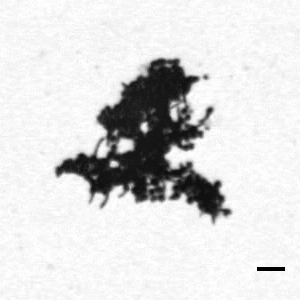
\includegraphics[width=5cm]{../C5/SporeAggregate}}
	\caption{An aggregate of \emph{A.~oryzae} spores sampled from a shake flask approximately 7~hours post-inoculation. Bar: \mic{25}.}
	\label{fig:SporeAgg}
\end{figure}

Given the limited growth of the mycelia presented here (Table~\ref{tab:VaryCMicroMorph}), the experiment was repeated in an attempt to analyse the microscopic form of the organism at a later point in time (24~hours post-inoculation). However, obtaining a large enough population of mycelia from which to derive a statistically relevant result, without sampling more than 10\% of the culture, was not feasible (data not shown). It is possible that as the mycelia increased in size, a degree of agglomeration occurred, further reducing the concentration of free mycelia in the media; agglomeration of \emph{A. oryzae} mycelia has previously been described by Amanullah and colleagues \cite{amanullah2001}. It was therefore concluded that microscopic examination of such cultures was not achievable and subsequent experimentation focussed on attempts to induce a greater degree of filamentous growth to enable quantification of micro-morphology.

\subsection{Influence of inoculum concentration on morphology and alpha-amylase production}

Increasing inoculum concentration has previously been demonstrated as an effective means of inducing filamentous growth in both \emph{A.~niger} \cite{papagianni2006a} and \emph{Rhizopus chinensis} \cite{teng2009}. As a dispersed growth form would permit a more extensive microscopic analysis, the effects of increasing the initial inoculum concentration above \inoc{1}{7} on morphology and $\alpha$-amylase production in the submerged fermentation of \emph{A.~oryzae} were investigated.

While pelleted biomass was found to predominate at all inoculum concentrations (and as a result, micro-morphological examination of \lq free' elements was not feasible), relationships between inoculum concentration ($C_i$), pellet diameter ($\Dp$) and $\alpha$-amylase yield were observed. $\alpha$-amylase activity per unit dry-cell weight (IU~mg\sp{-1}~DCW) appeared to be directly proportional to inoculum concentration ($R^2 = 0.95$; Fig.~\ref{fig:AmylasePelletInoc}), while mean pellet diameter was found to be inversely proportional to inoculum concentration ($R^2 = 0.96$).

\begin{figure}[htbp]
	\captionsetup[subfloat]{position=top}
	\centering
	\subfloat[]{\label{fig:AmylasePelletInoc}\pstool[width=10.3cm]{../C5/AmylasePelletInoc}{
		\psfrag{S}[Bc]{\al\hspace{1mm} $\alpha$-amylase activity per DCW (IU mg\sp{-1})}
		\psfrag{I}[Bc]{\al\hspace{2mm}$\Ci$ ($\times$ \sm{$10^7$})}
		\psfrag{M}[Bc]{\al\hspace{1mm} $\Dp$ (mm)}}
	}
	\\
	\subfloat[]{\label{fig:asDpCi}\pstool[width=10.3cm]{../C5/asDpCi}{
		\psfrag{S}[Bc]{\al\hspace{1mm} $\alpha$-amylase activity per DCW (IU mg\sp{-1})}
		\psfrag{M}[Bc]{\al\hspace{1mm} $\Dp$ (mm)}}
	}
	\caption{(a) $\alpha$-amylase activity per DCW ($\bs$) and mean pellet diameter ($\Dp$; $\bl$) versus inoculum concentration ($\Ci$) in the submerged fermentation of \emph{A. oryzae} 65 hours post-inoculation. (b) $\alpha$-amylase activity per DCW is inversely proportional to mean pellet diameter ($\Dp$). The dotted line represents Equation (\ref{eq:asDp}) with $\adx = 2.07$~IU~mm~mg\sp{-1} ($R^2 = 0.88$). Error bars represent standard deviation of two flasks. $\mbox{Spore viability} =35.7 \pm 7.1$\%.}
	\label{fig:Inoc}
\end{figure}

In an attempt to establish a preliminary link between metabolite yield and morphology, $\alpha$-amylase activity per DCW was expressed as a function of $\Dp$ (Fig.~\ref{fig:asDpCi}), which is derived from the measured projected area ($\Ap$; mm\sp{2}) of each pellet by calculating the equivalent radius ($r = \sqrt{\Ap\pi^{-1}}$). Given the evidence in the literature for metabolite excretion occurring primarily at hyphal tips \cite{gordon2000,muller2002} and productive biomass being limited to the outer layer of pellets \cite{pirt1966,elenshasy2006}, it seems reasonable that $\alpha$-amylase activity per DCW would be directly proportional to the mean pellet surface area times the number of pellets present in the media ($n$):

\begin{equation} \label{eq:asnr}
	\hbox{$\alpha$-amylase activity per DCW} \propto n4\pi r^2 
\end{equation}

\noindent This is based on the assumption that the product of the number of hyphal tips ($N$) per unit area of pellet surface and the amount of $\alpha$-amylase produced by each tip is relatively independent of inoculum concentration:

\begin{equation}\label{eq:aaNA}
	\frac{\hbox{$\alpha$-amylase activity}}{N} \times \frac{N}{4 \pi r^2} = c
\end{equation}

\noindent where $c$ is a constant. For a given level of biomass, $n$ is inversely proportional to pellet size (or pellet volume):

\begin{equation} \label{eq:nr}
	n \propto \frac{1}{\frac{4}{3}\pi r^3} 
\end{equation}

\noindent Combining equations~\ref{eq:asnr} and \ref{eq:nr} and substituting for $r$:

\begin{equation} \label{eq:asDp}
	\hbox{$\alpha$-amylase activity per DCW} = \frac{\adx}{\Dp}
\end{equation}

\noindent where $\adx$ (IU~mm~mg\sp{-1}) is a proportionality constant. This relationship is illustrated graphically in Figure~\ref{fig:asDpCi}.

These results are in general agreement with reports in the literature that suggest a low inoculum concentration results in larger pellets \cite{papagianni2002,papagianni2006a,dobson2008b} and that smaller pellets result in higher metabolite yields in \emph{Aspergilli} \cite{elenshasy2006,couri2003,ali2006,xu2000}. While a correlation between pellet size and $\alpha$-amylase production appeared to exist in this study, the microscopic examination of pellets using light microscopy was not feasible, due to their three-dimensional structure and relatively large size ($\Dp \leq 7$~mm). The potential for obtaining micro-morphological insights into enzyme production using inoculum concentration as a process variable was therefore deemed to be limited.

\subsection{Influence of surfactant compounds on morphology and metabolite yield}

During the course of this work, studying \emph{A. oryzae} at the microscopic level was often complicated by the lack of \lq free' mycelia present in submerged culture due to the agglomerative nature of the organism's conidiospores. However, several studies have reported successful attempts to regulate morphology by supplementing media with various polymers and surfactant (surface active agent) compounds \cite{znidarsic2000,domingues2000,dobson2008b,lucatero2004,ilic2008}. The effect of some of these substances on cultures of \emph{A. oryzae} was therefore investigated.

\subsubsection{Influence of Tween-80 on morphology and $\alpha$-amylase production}

In an attempt to counteract the agglomeration of spores, without adversely affecting growth or metabolite production, Tween-80, a surfactant routinely used in fungal conidial preparations to aid spore dispersal, was incorporated into submerged culture and its impact on morphology and $\alpha$-amylase yield was quantified. The addition of 0.05\% (w/v) Tween-80 resulted in an increase in $\alpha$-amylase activity of approximately 59\% in flasks inoculated with \inoc{1}{8} (Fig.~\ref{fig:aaDCWT80}); further increasing the concentration of Tween-80 up to 0.56\% (w/v) had little additional effect. In flasks inoculated with \inoc{1}{7}, $\alpha$-amylase activity was slightly reduced in the presence of 0.05\% (w/v) Tween-80, but increasing the concentration to 0.25\% (w/v) resulted in an increase in activity of approximately 47\%. Biomass levels appeared to be relatively independent of Tween-80 concentration.

\begin{figure}[tb]
	\centering
	\pstool[width=10.5cm]{../C5/aaDCWT80}{
		\psfrag{A}[Bc]{\al\hspace{1mm} DCW (\omgml);}
		\psfrag{a}[Bc]{\al\hspace{1mm} $\alpha$-amylase activity (\IUml)}	
		\psfrag{T}[Bc]{\al\hspace{3mm} \% Tween-80 (w/v)}}
	\caption{Impact of supplementing \emph{Aspergillus oryzae} fermentation broth with Tween-80 on $\alpha$-amylase activity ($\bl$, $\lozenge$) and dry cell weight ($\bs$, $\square$) for inoculum concentrations of $1 \times 10^7$ ($\bl$, $\bs$) and \inoc{1}{8} ($\lozenge$, $\square$) 65~hours post-inoculation. Error bars represent standard deviation of two flasks. $\mbox{Spore viability} = 52.8 \pm 11.7$\%.}
	\label{fig:aaDCWT80}
\end{figure}

The addition of 0.05\% (w/v) Tween-80 resulted in a significant increase in pellet size at the lower inoculum concentration (Fig.~\ref{fig:DpT80}), which may explain the observed reduction in $\alpha$-amylase activity at this concentration. However, despite producing slightly larger pellets, flasks inoculated with \inoc{1}{8} produced higher yields of $\alpha$-amylase per DCW in the presence of Tween-80. This complex relationship is emphasised in Figure (\ref{fig:asDpT80}), where no clear correlation between pellet size and $\alpha$-amylase activity per DCW is apparent ($R^2 = 0.52$ for linear regression).

\begin{figure}[htbp]
	\centering
	\captionsetup[subfloat]{position=top}
	\subfloat[]{\label{fig:DpT80}\pstool[width=10.5cm]{../C5/DpT80}{
		\psfrag{M}[Bc]{\al $\Dp$ (mm)}
		\psfrag{T}[Bc]{\al\hspace{2mm} \% Tween-80 (w/v)}}
	}
	\\
	\subfloat[]{\label{fig:asDpT80}\pstool[width=10.5cm]{../C5/asDpT80}{
		\psfrag{M}[Bc]{\al $\Dp$ (mm)}
		\psfrag{S}[Bc]{\al $\alpha$-amylase activity per DCW (IU mg\sp{-1})}}
	}
  \caption{Impact of supplementing \emph{Aspergillus oryzae} fermentation broth with Tween-80 on (a) mean pellet diameter ($\Dp$) after 65 hours' incubation for inoculum concentrations of $1 \times 10^7$ ($\bs$) and \inoc{1}{8} ($\bl$). (b) No direct relationship between $\alpha$-amylase activity per DCW and $\Dp$ was found. Error bars represent standard deviation of two flasks. $\mbox{Spore viability} = 52.8 \pm 11.7$\%.}
\end{figure}

The higher yield of $\alpha$-amylase obtained in the presence of Tween-80 may be evidence of an influence at the micro-morphological level, such as an increase in hyphal branching. A microscopic analysis of pellets (Fig.~\ref{fig:PelletsT80}) suggests that this is not the case, as similar values of circularity ($C = 4 \pi \Ap P^{-2}$) were obtained for pellets cultivated with or without Tween-80 supplementation (Table~\ref{tab:TweenPelletMorph}). However, a more extensive microscopic examination was required to generate a more conclusive result.

\begin{table}[tb]
	\centering
	\footnotesize
	\caption{Mean projected area ($\Ap$) and mean circularity ($C$) of \emph{A. oryzae} pellets 24~hours post-inoculation when cultivated in media supplemented with Tween-80 as indicated. Flasks were inoculated with \inoc{1}{7} ($\mbox{viability} = 35.5$\%) and incubated at \celc{30}. Errors represent 95\% confidence intervals.}
	\label{tab:TweenPelletMorph}
	\begin{tabularx}{(\textwidth - 1cm)}{X X X r}
		\toprule
		Tween-80 (\% w/v) & $\Ap$ (\mics{$\times 10^6$}) & $C$ & $n$ \\
		\midrule
		0.0 & $1.50 \pm 0.28$ & $0.032 \pm 0.007$ & 12\\
		0.5 & $1.28 \pm 0.28$ & $0.028 \pm 0.005$ & 12\\
		1.0 & $1.51 \pm 0.25$ & $0.027 \pm 0.004$ & 10\\
		\bottomrule
	\end{tabularx}
\end{table}

\begin{figure}[hbtp]
	\centering
	\captionsetup[subfloat]{justification=centerlast}
	\subfloat[\mics{$\Ap = 1.68 \times 10^6$}, $C = 0.027$]{\label{fig:Pellet00T80}\fbox{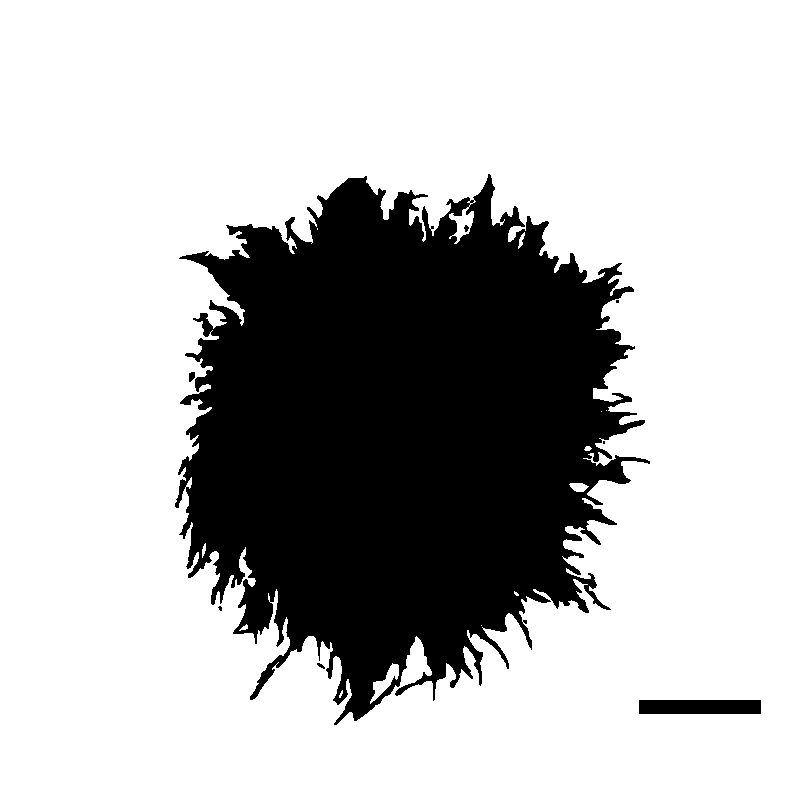
\includegraphics[width=5cm]{../C5/Pellet00T80}}}
	\hspace{0.5cm}
	\subfloat[\mics{$\Ap = 1.64 \times 10^6$}, $C = 0.025$]{\label{fig:Pellet10T80}\fbox{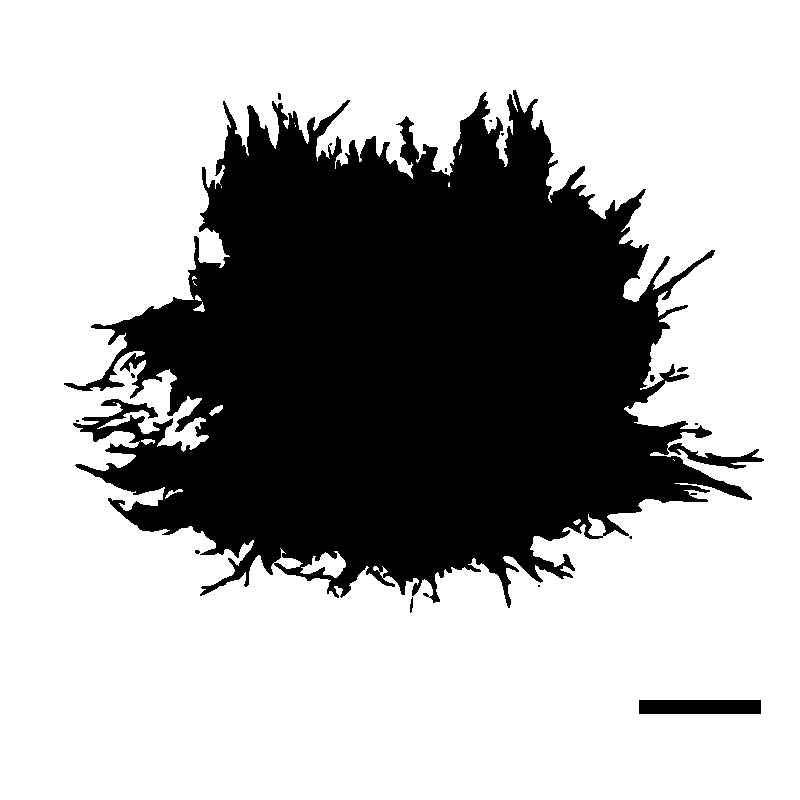
\includegraphics[width=5cm]{../C5/Pellet10T80}}}
  \caption{Morphology of \emph{A. oryzae} pellets cultivated in the presence of (a) 0\% and (b) 1.0\% (w/v) Tween-80. Cultivation conditions were as described in Table~\ref{tab:TweenPelletMorph}. Bars: 0.4~mm.}
  \label{fig:PelletsT80}
\end{figure}

\subsubsection{Influence of Tween-80 on micro-morphological development in solid culture}

The effect of Tween-80 on the early-stage, microscopic development of \emph{A. oryzae} was investigated on solid substrate using membrane-immobilisation in order to isolate individual mycelia for subsequent image analysis. The inclusion of Tween-80 in the media resulted in a small decrease in the hyphal growth unit compared to the control, although this decrease was not statistically significant (Fig.~\ref{fig:LhguT80}). Furthermore, given the reasonable correlation between $\hgu$ and $\Lh$ evident in Figure~\ref{fig:MicroT80}, it is probable that this lower value of $\hgu$ was related to a decrease in the extent of growth, rather than any change in the morphology of the organism (Fig.~\ref{fig:ThlNtT80}). It was therefore concluded that no appreciable influence of Tween-80 on hyphal extension was evident, but the increase in pellet size observed at some concentrations in submerged culture was still without explanation.

\begin{figure}[htbp]
	\captionsetup[subfloat]{position=top}
	\centering
	\subfloat[]{\label{fig:LhguT80}\pstool[width=10.5cm]{../C5/LhguT80}{
		\psfrag{H}[Bc]{\al $\hgu$ (\omic)}
		\psfrag{T}[Bc]{\al \hspace{2mm} \% Tween-80 (w/v)}}
	}
	\\
	\subfloat[]{\label{fig:ThlNtT80}\pstool[width=10.5cm]{../C5/ThlNtT80}{
		\psfrag{H}[Bc]{\al $\Lh$ (\omic)}
		\psfrag{T}[Bc]{\al \hspace{2mm} \% Tween-80 (w/v)}
		\psfrag{N}[Bc]{\al $N$}}
	}
	\caption{Variation in (a) the mean hyphal growth unit ($\hgu$) and (b) the mean total hyphal length ($\Lh$; $\bl$) and mean number of tips ($N$; $\bs$) of populations of \emph{Aspergillus oryzae} mycelia cultivated on malt agar supplemented with varying concentrations of Tween-80 (\celc{30}, 20~h). Error bars represent 95\% confidence intervals.}
	\label{fig:MicroT80}
\end{figure}

\subsubsection{Effect of Tween-80 on spore agglomeration}

The observed influence of Tween-80 on pellet diameter (Fig.~\ref{fig:DpT80}) was investigated at the microscopic level by assessing the effect of the surfactant on particle agglomeration. Approximately 2 hours post-inoculation, the number of particles present in the media was up to 45\% higher in the presence of the Tween-80, the difference being even more pronounced at 4 hours post-inoculation (Fig.~\ref{fig:AggT}). The lower of the two Tween-80 concentrations (0.05\% w/v) resulted in a greater degree of dispersal, but from 6 hours onwards, there was no significant difference in particle dispersal between the three different media, suggesting that any impact was short-lived.

\begin{figure}[tb]
	\centering
	\pstool[width=10.5cm]{../C5/AggT}{
		\psfrag{A}[Bc]{\al Number of objects (\ml{$\times 10^4$})}
		\psfrag{T}[Bc]{\al \hspace{2mm} Time (h)}}
	\caption{Time-course of aggregation in the submerged fermentation of \emph{Aspergillus oryzae} in the presence of 0 ($\bs$),  0.05 ($\bl$) and 0.1 ($\bt$) \% Tween-80 (w/v). All flasks inoculated with \inoc{2}{7}. Error bars represent standard deviation of two flasks, with approximately 27 fields of view examined for each flask.}
	\label{fig:AggT}
\end{figure}

There is evidence that suggests the surface properties of fungal spores are altered during the swelling and germination process. Investigations using atomic force microscopy have shown that the hydrophobicity of \emph{A. oryzae} and \emph{A. fumigatus} conidia decreases as they swell and germinate \cite{vanderaa2002,dague2008}. This may offer an explanation as to why the influence of Tween-80 does not seem to be visible 6 hours post-inoculation.

\subsubsection{Does Tween-80 influence the morphology of \emph{Aspergillus oryzae}?}

Based on the series of investigations conducted here, it was concluded that Tween-80 had a limited influence on pellet formation in submerged cultures of \emph{A. oryzae}. Although Tween-80 has been found to inhibit pellet formation in \emph{T. reesei} \cite{domingues2000}, it has also been found to cause an increase in pellet size in cultures of \emph{R. nigricans} \cite{znidarsic2000}, although in the case of the latter, a degree of filamentous growth was also induced at higher concentrations. However, no inducement of filamentous growth was observed here and, as such, a thorough microscopic examination of submerged culture was not possible, and no relationship between the increase in $\alpha$-amylase production and micro-morphological parameters (such as $\hgu$) was obtainable. Subsequent experimentation focussed on investigations of other surfactants and polymers that had been previously reported to inhibit pellet formation.

\subsubsection{Further qualitative assessment of the morphological influence of polymers and surfactants}

The potential of a number of other polymers and surfactant compounds to disrupt pellet formation in cultures of \emph{A. oryzae} was investigated. The majority of compounds tested resulted in the formation of pellets of either smaller (Ficoll) or larger diameter (diethylaminoethyl cellulose, Sephadex G-75) than the control (data not shown). However, other compounds seemed to inhibit pellet formation to some extent, producing filamentous structures (together with pellets) that were potentially suited to routine microscopic analysis (Fig.~\ref{fig:PolyDetMorph}). However, polymers such as carboxymethylcellulose (CMC) and Sephadex caused the media to exhibit a paste-like consistency, which complicated dry-cell weight determination and for this reason they were deemed unsuitable for further study. Subsequent experiments examined the effect of the non-ionic detergents, Triton X-100 and Nonidet P-40.

\begin{figure}[hbtp]
	\centering
	\subfloat[]{\label{fig:TX100Morph}\fbox{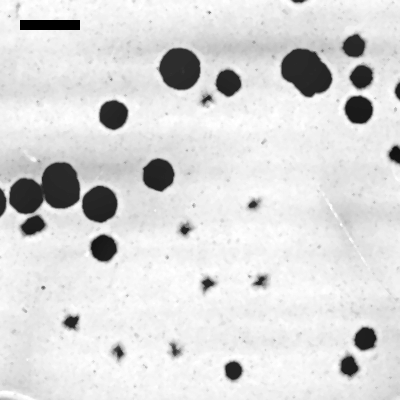
\includegraphics[width=4cm]{../C5/TX100Morph}}}
	\hspace{0.5cm}
	\subfloat[]{\label{fig:CMCMorph}\fbox{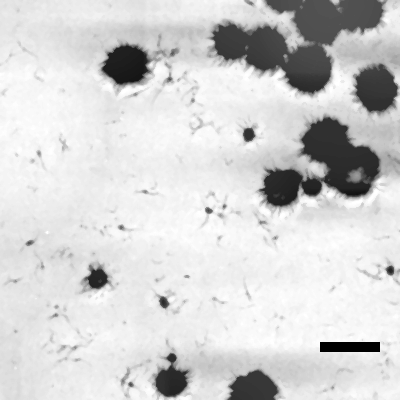
\includegraphics[width=4cm]{../C5/CMCMorph}}}
	\hspace{0.5cm}
	\subfloat[]{\label{fig:SG200Morph}\fbox{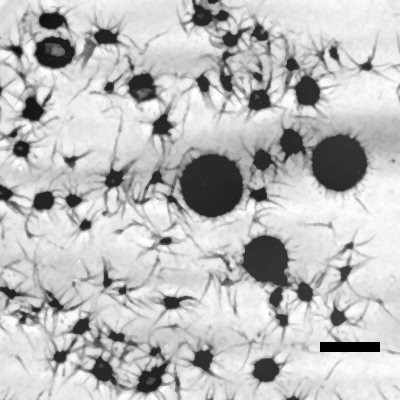
\includegraphics[width=4cm]{../C5/SG200Morph}}}
  \caption{Variation in morphology of \emph{A. oryzae} after 72 hours resulting from supplementation with 0.6\% w/v (a) Triton X-100, (b) carboxymethylcellulose and (c) Sephadex G-200. Bars: 5~mm.}
  \label{fig:PolyDetMorph}
\end{figure}

\subsubsection{Influence of Triton X-100 and Nonidet P-40 on macro-morphology and metabolite yield}

The addition of 0.1\% (w/v) Triton X-100 resulted in an increase of approximately 149\% in $\alpha$-amylase activity; higher concentrations had no further effect (Fig.~\ref{fig:aaDCWDet}). The addition of Triton X-100 also caused a reduction in biomass levels of up to 51\%, resulting in increases in $\alpha$-amylase per DCW of up to 184\%. Lower biomass yields may suggest a negative physiological impact of the detergent and an inhibition of growth. The addition of Nonidet P-40 caused similar reductions in biomass levels, but the resultant increases in $\alpha$-amylase activity were significantly less.

\begin{figure}[htbp]
	\captionsetup[subfloat]{position=top}
	\centering
	\subfloat[]{\label{fig:aaDCWDet}\pstool[width=10cm]{../C5/aaDCWDet}{
		\psfrag{A}[Bc]{\al DCW (\omgml);}
		\psfrag{a}[Bc]{\al $\alpha$-amylase activity (\IUml)}
		\psfrag{D}[Bc]{\al\hspace{2mm} \% Detergent (w/v)}}
	}
	\\
	\subfloat[]{\label{fig:asDpDet}\pstool[width=10cm]{../C5/asDpDet}{
		\psfrag{S}[Bc]{\al $\alpha$-amylase per DCW (IU mg\sp{-1} DCW)}
		\psfrag{M}[Bc]{\al $\Dp$ (mm)}}
	}
	\caption{(a) Impact of supplementing \emph{Aspergillus oryzae} fermentation broth with different concentrations of Nonidet P-40 ($\bs$, $\bl$) and Triton X-100 ($\square$, $\lozenge$) on $\alpha$-amylase activity ($\bl$, $\lozenge$) and dry cell weight (DCW; $\bs$, $\square$). Average of two independent results is shown. Error bars represent standard deviation. (b) Mean pellet diameter ($\Dp$) versus $\alpha$-amylase activity per unit dry cell weight in the presence of Nonidet P-40 ($\bl$), Triton X-100 ($\bs$) and without supplementation ($\bullet$). All flasks inoculated with \inoc{9}{6} ($\mbox{viability} = 45.3 \pm 2.9$\%).}
\end{figure}

In the case of both Nonidet P-40 and Triton X-100, no correlation was found between $\alpha$-amylase per DCW and pellet size (Fig.~\ref{fig:asDpDet}). Evidence in the literature suggests that smaller pellets should result in a higher metabolite yield \cite{dobson2008b,elenshasy2006,couri2003,ali2006,xu2000}, but $\alpha$-amylase activity was lower in flasks supplemented with Nonidet P-40 compared to those supplemented with Triton X-100 (but still higher than the control), even though the latter produced larger pellets. This may be explained by the lower dry-cell weights observed in the presence of detergents; the smaller pellet sizes may be partly caused by inhibition of growth rather than dispersal of biomass. Evidently, a macro-morphological analysis alone is not sufficient to explain the effect of non-ionic detergents on \emph{A. oryzae}.

The detergents may have had a micro-morphological effect; an increase in hyphal branching may have been responsible for the observed increase in $\alpha$-amylase yield. However, microscopic examination of the fungus in the presence of either Triton X-100 or Nonidet P-40 was not possible, as samples taken from these fermentations exhibited poor stain uptake (lactophenol cotton blue; not shown). Whether this was a result of an inhibition of staining by the detergents, or a physiological influence of the detergents on the cells, resulting in variations in cell wall composition, is not clear. Alternatively, it is possible that the presence of non-ionic detergents in the media caused an increase in cell permeability, leading to greater mass diffusion into the pellets \cite{domingues2000,znidarsic2000}. This may have resulted in a wider \lq active' region in the pellet, causing an increase in metabolite production. The increase in $\alpha$-amylase activity observed in the presence of non-ionic detergents may also have been a result of enhanced activation of the enzyme by the surfactants, rather than an increase in enzyme production by \emph{A. oryzae}. Supplementing a solution containing porcine pancreatic $\alpha$-amylase with 0.02\% w/v Triton X-100 has been shown to result in an increase in activity of approximately 40\% \cite{yoon2005}.